\section{RNG\_\-UNIFORM\_\-INT Class Reference}
\label{classRNG__UNIFORM__INT}\index{RNG_UNIFORM_INT@{RNG\_\-UNIFORM\_\-INT}}
{\tt \#include $<$rng\_\-uniform\_\-int.h$>$}

Inheritance diagram for RNG\_\-UNIFORM\_\-INT::\begin{figure}[H]
\begin{center}
\leavevmode
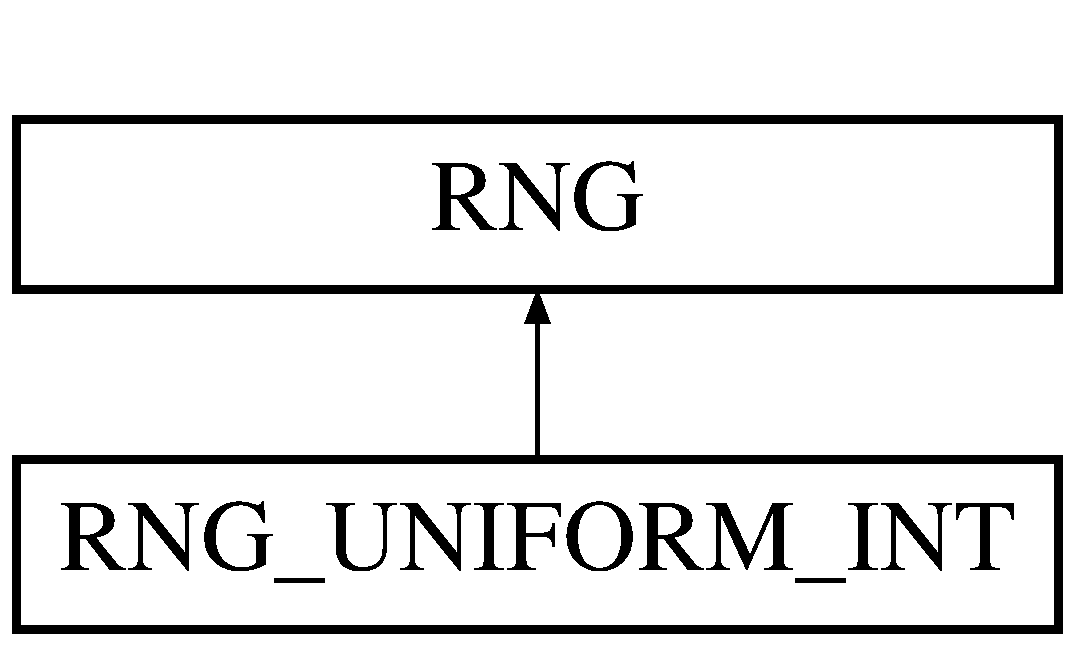
\includegraphics[height=2cm]{classRNG__UNIFORM__INT}
\end{center}
\end{figure}
\subsection*{Public Member Functions}
\begin{CompactItemize}
\item 
\textbf{RNG\_\-UNIFORM\_\-INT} (const gsl\_\-rng\_\-type $\ast$, const unsigned long)\label{classRNG__UNIFORM__INT_058d4b1ce58e8a2324fbcd97c8fe99a4}

\item 
\textbf{RNG\_\-UNIFORM\_\-INT} (const gsl\_\-rng\_\-type $\ast$, const unsigned long, const unsigned long)\label{classRNG__UNIFORM__INT_470ef4868fb284074ece8e046dec8b12}

\item 
virtual long double \textbf{Get} ()\label{classRNG__UNIFORM__INT_752287963156809b16d68705424c703d}

\end{CompactItemize}
\subsection*{Protected Attributes}
\begin{CompactItemize}
\item 
unsigned long \textbf{max}\label{classRNG__UNIFORM__INT_3e2c830285eacf4fe69b2579fc1c2f02}

\end{CompactItemize}


\subsection{Detailed Description}
\begin{Desc}
\item[Author:]Krishnan S \end{Desc}




The documentation for this class was generated from the following files:\begin{CompactItemize}
\item 
rng\_\-uniform\_\-int.h\item 
rng\_\-uniform\_\-int.cpp\end{CompactItemize}
